\documentclass[a4paper,12pt]{article} % This defines the style of your paper

\usepackage[top = 2.5cm, bottom = 2.5cm, left = 2.5cm, right = 2.5cm]{geometry} 

\usepackage[T1]{fontenc}
\usepackage[utf8]{inputenc}

\usepackage{multirow} % Multirow is for tables with multiple rows within one cell.
\usepackage{booktabs} % For even nicer tables.

\usepackage{graphicx} 
\usepackage{tikz}
\usepackage{xcolor}

\usepackage{setspace}
\setlength{\parindent}{0in}

\usepackage{float}

\usepackage{fancyhdr}


\pagestyle{fancy} % With this command we can customize the header style.

\fancyhf{} % This makes sure we do not have other information in our header or footer.

\rhead{\footnotesize J. Klepl}

\cfoot{\footnotesize \thepage} 

\begin{document}

\thispagestyle{empty} % This command disables the header on the first page. 

\begin{center}
	{\Large \bf Homework 3 - splay\_experiment}
	\vspace{2mm}
	
	{\bf Jiří Klepl}
		
\end{center}  

\vspace{0.4cm}


\setlength{\parindent}{2em}

\subsection*{Prolog}

Následují diskuze tří zadaných testů a analýzy pozorovaných domnělých závislostí. Pro úvod by bylo vhodné říct, že všechny testy měří a průměrují počet provedených rotací naivní a standardní implementace splay stromu. Tento test je poměrně dobrým měřítkem časové složitosti práce nad těmito strukturami, neboť u splay stromů počet rotací odpovídá počtu čtení a dereferencí prvků, které vedou k přidanému/hledanému prvku (právě přidání a hledání prvku testy měří).

\subsection*{Sequential test}

\begin{figure}[!htb]
    \caption{Sequential test results}
    \label{seq_results}
    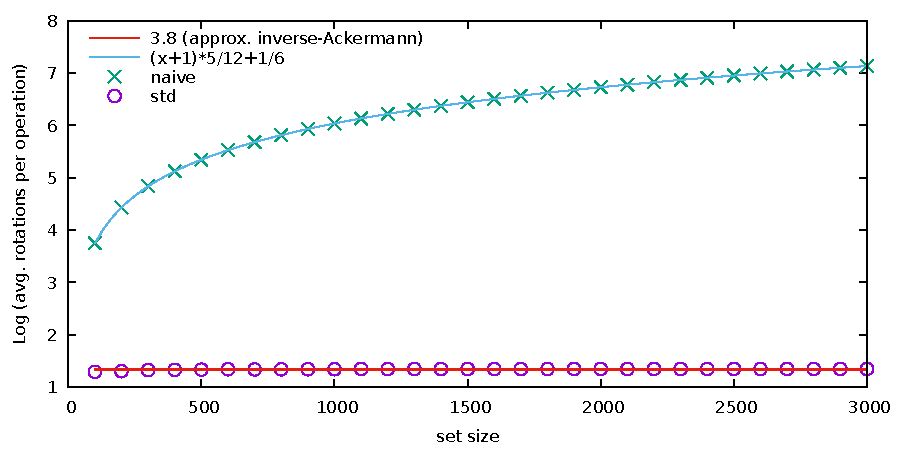
\includegraphics{sequential.pdf}    
\end{figure}

Ve výsledcích tohoto testu znázorněných ve figuře \ref{seq_results} můžeme vidět velký rozdíl v počtu provedených rotací naivní a standardní implementace.

U obou implementací je složitost přidávání $n$ prvků v $\Theta(n)$, tedy konstantní na jeden prvek. Výsledkem je vždy lineární seznam (při vzestupném přidávání propojen po levých synech). Tento výsledný tvar budou mít obě implementace po každém dokončení (přidávací/hledací) sekvence.

Složitost hledání prvku v naivní implementaci je v $\Theta(n)$. Strom má během hledání vždy tvar dvou hlavami spojených seznamů, z nichž jednomu odtrháváme listy a přidáváme je v hlavě do druhého. Jednoduchou matematickou úpravou proto dostaneme velice přesnou lineární aproximaci závislosti průměrného počtu rotací na velikosti pole.

Složitost hledání prvku ve standardní implementaci je v $\Theta(\alpha(n))$, kde $\alpha$ je inverzní Ackermannova funkce, důkaz toho lze nalézt na internetu. Tato analýza odpovídá mazání krajních bodů, když splay stromem reprezentujeme deque.

\pagebreak

\subsection*{Random test}

\begin{figure}[!htb]
    \caption{Random test results}
    \label{rng_results}
    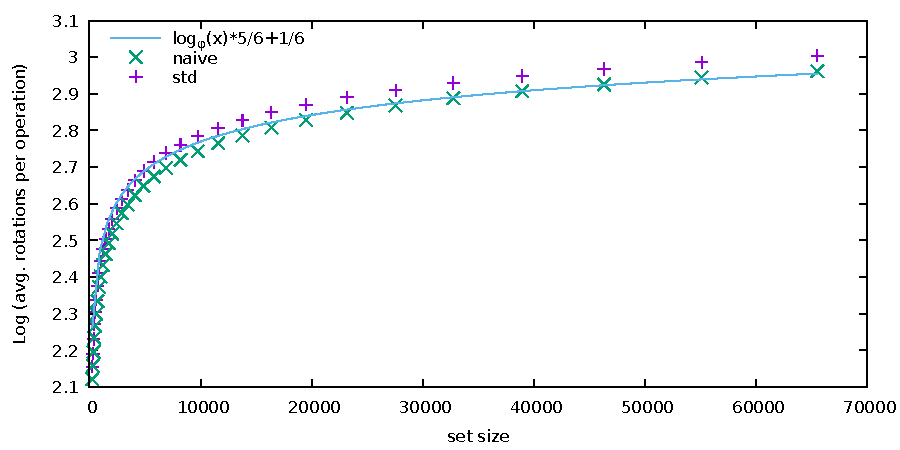
\includegraphics{random.pdf}    
\end{figure}

V testu s náhodným přístupem k prvkům dosahují obě implementace obdobného počtu rotací (pozn. znázorněná funkce je pouze k porovnání, není výsledkem žádné analýzy), na jeden prvek amortizovaně v $\Theta(n)$ (kde $n$ je počet prvků). U standardní implementace toto není vůbec překvapivé, na přednáškách to bylo rigorózně dokázáno.

Jediným překvapením zde je podobnost výsledků naivní a standardní implementace. V dalším testu najdeme vysvětlení, které by částečně mohlo vysvětlovat i toto (včetně toho, proč naivní implementace dává lepší výsledky). Ono vysvětlení však zde není uspokojivé.

Co nám dá vysvětlení logaritmického počtu rotací je, že v libovolném nevyváženém podstromě budeme pravděpodobněji vyrotovávat prvky z větší (mohutnější) strany (na figuře \ref{rot} to je levá $(a, A_1, A_2)$). Když tedy budeme uvažovat tomu odpovídající rotaci prvku $a$, tak prvky z $A_1$ posuneme výš, prvky $B$ z níž a prvky z $A_2$ budou stále ve stejné výšce, sníží se velikost levého podstromu a pravděpodobnost přístupu k jeho prvkům, opačně s pravým podstromem. Tedy naivní splay stromy se mají tendenci samy vyvažovat. A pak tedy tradičně podle průměrné hloubky.

\begin{figure}[!htb]
    \caption{Rotation}
    \centering
    \label{rot}
\usetikzlibrary{shapes}
\usetikzlibrary{shapes.geometric,positioning}
\begin{tikzpicture}[nodes={draw, circle}, ->]
 
\begin{scope}[xshift=-3cm]
    \node{$r$}
    child { node {$a$} 
        child { node[above=-2cm,xshift=-0.5cm,shape border uses incircle,
        isosceles triangle,isosceles triangle apex angle=45,
        shape border rotate=90, draw] {$A_1$} }
        child{ node[above=-2cm,xshift=0.5cm,shape border uses incircle,
        isosceles triangle,isosceles triangle apex angle=45,
        shape border rotate=90, draw]{$A_2$} }
    }
    child{ node[above=-1cm,shape border uses incircle,
    isosceles triangle,isosceles triangle apex angle=45,
    shape border rotate=90, draw]{$B$} };
\end{scope}
 
\begin{scope}[xshift=3cm]
    \node{$a$}
    child { 
        node[above=-2cm,xshift=-1cm,shape border uses incircle,
        isosceles triangle,isosceles triangle apex angle=45,
        shape border rotate=90, draw] {$A_1$}
    }
    child{ node {$r$} 
        child{ node[above=-2cm,xshift=-0.5cm,shape border uses incircle,
        isosceles triangle,isosceles triangle apex angle=45,
        shape border rotate=90, draw]{$A_2$} }
        child { node[above=-1cm,shape border uses incircle,
        isosceles triangle,isosceles triangle apex angle=45,
        shape border rotate=90, draw]{$B$} }
    };
\end{scope}
 
\end{tikzpicture}
\end{figure}


\pagebreak

\subsection*{Subset test}

\begin{figure}[!htb]
    \caption{Subset test results}
    \label{subset_results}
    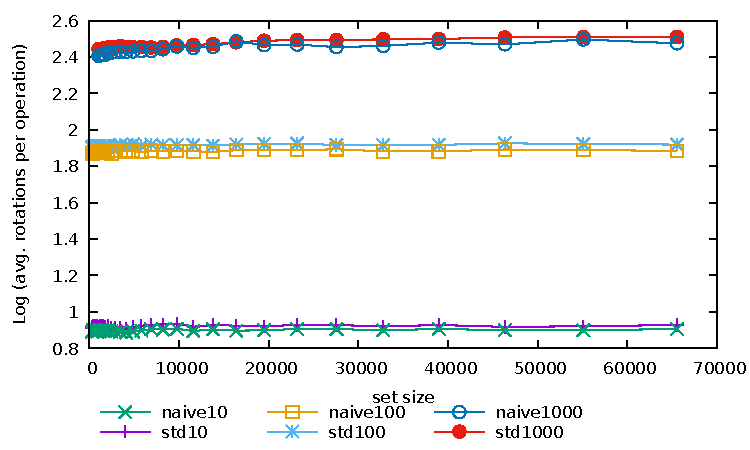
\includegraphics{subset2d.pdf}    
\end{figure}

V testu s náhodným přístupem do malé množiny prvků uvnitř velké množiny přidaných prvků opět vidíme velice podobný počet provedených rotací naivní a standardní implementace (pro danou konfiguraci testu).

Dále vidíme, že velikost stromů nemá v tomto testu signifikantní vliv na počet rotací. Naproti tomu velikost navštěvované podmnožiny má stejný vliv jako ona velikost v minulém testu (kde totiž velikost stromu odpovídala velikosti přistupované podmnožiny).


\subsubsection*{Vysvětlení pro naivní implementaci}

Snažíme se vysvětlit, proč nemá velikost nadmnožiny vliv na práci se stromem a důležitá je jen přistupovaná podmnožina.

Uvažujme \textbf{``podmnožinovou špičku'' stromu} (budeme značit $A_i$, či neformálně $A$; $i$ značí počet provedených přístupů), což je v kořeni začínající maximální spojitý podgraf prvků, které jsou v podmnožině. (pozn. $A_0$ nemá smysl uvažovat, byl by prázdný, ale $A_1$ je poté alespoň kořen).

Špička $A$ je (z definice) vždy spojitá a obsahuje prvky pouze z podmnožiny, tedy je-li přistupovaný prvek v tomto podgrafu, nikdy ani nesáhneme na prvek, který by v $A$ nebyl (pozn. rotace neuvede na cestu od prvku z $A$ ke kořeni prvek, který by nebyl z $A$). Tedy zbytek stromu je irelevantní při přistupování k prvkům z $A$.

Teď jen ukážeme, že prvky $A_i$ jsou i v $A_{i+1}$. Nikdy nenastane vyrotovávání prvku, který není z $A$. Tedy jediná relevantí situace je, když vyrotovávaný prvek (nutně z podmnožiny) je těsně pod $A$ (jinak se nic nerozbíjí, protože jsme v nějakém podstromě až dále pod $A$ a na žádný prvek z $A$ v rotacích nesáhneme). První situace, kdy vyrotovávaný prvek (který ještě není v $A$) manipuluje s nějakým prvkem z $A$, je, když už v $A$ sám je (neboť manipuluje jen se svým rodičem), tedy jeho rodič je nutně v $A$. Tedy jakákoliv snaha o rozbití množiny $A$ by nám dala spor.

Předešlé dva odstavce nám dohromady dají, že přistoupíme-li k prvkům z nějaké podmnožiny a poté nepřistoupíme k žádnému jinému a poté opět přistoupíme k prvkům z této podmnožiny, tak již vůbec nesáhneme na prvek, který by nebyl v této podmnožině.

\subsubsection*{Vysvětlení pro standardní implementaci}

Pro standardní splay strom vysvětlení naivní implementace platí jen, když připustíme ``skoro spojitost'' výše zmíněné špičky $A$. Tedy připustíme, aby na cestě mezi prvkem v $A$ a jeho prvním předkem z $A$ byl maximálně jeden prvek, který není v podmnožině. Problematické totiž jsou \textit{zigzig} rotace.

zig rotace a zigzag rotace nijak neohrožují špičku $A$, stále pro ně platí naivní vysvětlení. Zigzag rotace jediná může ``Vytrhnout'' prvek z $A$ a nahradit jej vyrotovávaným, jenže ten je taktéž z podmnožiny a díky připuštění ``skoro spojitosti'' je vytrhnutý prvek stále v $A$.

Maximální vliv nadmnožiny je tedy určitě omezen dvojnásobkem vlivu podmnožiny, tedy nadmnožina asymptoticky významná není a i tohoto dvojnásobku docílíme jen ve velice konkrétních situacích a většinou bude špička $A$ poměrně podobná špičce naivní implementace (pozn. $A$ se nikdy nezhoršuje, pokud se konkrétně přes její hranici neprozigziguje nový prvek $A$ - toto je jediný možný způsob uvedení mezery do $A$, ostatní rotace ji jistě nezhoršují).

Tyto mezery v $A$ pravděpodobně vysvětlují v grafu viditelný nepatrný rozdíl implementací.

\end{document}